\chapter{线程中}
课前思考
\begin{enumerate}
	\item 多线程是如何实现同步的?
	\item 多线程中如何避免死锁问题?
	\item 线程的生命周期是怎么样的?
	\item 多个线程之间优先级如何控制?
\end{enumerate}
学习目标
\begin{enumerate}
	\item java中多线程的同步控制方法
	\item 掌握线程的生命周期
	\item 理解多线程同步的锁机制和线程优先级
\end{enumerate}
\section{线程同步的思路}
\subsection{多线程的同步控制}
\begin{itemize}
	\item 有时线程之间彼此不独立,需要同步
	\subitem 线程间的互斥:
	\subsubitem 同时运行的几个线程需要共享一些数据
	\subsubitem 共享的数据,在某个时刻只允许一个线程对其进行操作
	\subitem “生产者/消费者”问题
	\subsubitem 假设一个线程负责往数据区写数据,另一个线程从同一数据区读数据,两个线程并行执行
	\subsubitem 如果数据区已满,生产者要等消费者取走一些数据后才能再写
	\subsubitem 当数据去为空,消费者要等生产者写入一些数据后再取
\end{itemize}
\begin{lstlisting}[language=java]
//Ticket.java
public class Ticket {
	int number = 0;
	int size;
	boolean available = false;
	public Ticket(int size) {
		this.size = size;
	}
}
//Producer.java
public class Producer extends Thread {
	Ticket t = null;
	public Producer(Ticket t) {
		this.t = t;
	}
	public void run() {
		while (t.number < t.size) {
			System.out.println("Producer puts ticket " + (++t.number));
			t.available = true;
		}
	}
}
//Consumer.java
public class Consumer extends Thread {
	Ticket t = null;
	int i = 0;
	public Consumer(Ticket t) {
		this.t = t;
	}
	public void run() {
		while (i < t.size) {
			if (t.available == true && i <= t.number) {
				System.out.println("Consumer buys ticket " + (++i));
			}
			if (i == t.number) {
				t.available = false;
			}
		}
	}
}
//Machine.java
public class Machine {
	public static void main(String[] args) {
		Ticket t = new Ticket(10);
		new Consumer(t).start();
		new Producer(t).start();
	}
}
//output
Producer puts ticket 1
Producer puts ticket 2
Consumer buys ticket 1
Producer puts ticket 3
Consumer buys ticket 2
Producer puts ticket 4
Consumer buys ticket 3
Producer puts ticket 5
Consumer buys ticket 4
Producer puts ticket 6
Producer puts ticket 7
Producer puts ticket 8
Consumer buys ticket 5
Producer puts ticket 9
Producer puts ticket 10
Consumer buys ticket 6
Consumer buys ticket 7
Consumer buys ticket 8
Consumer buys ticket 9
Consumer buys ticket 10
\end{lstlisting}
如果将line 35-line37改为下面代码,因为当消费者休眠时,CPU执行生产者t.available=true,但当消费者休眠完毕,将会设置t.available=true,
因此会导致程序一直运行。
\begin{lstlisting}[language=java]
if (i == t.number) {
	try {
		Thread.sleep(1);
	} catch (InterruptedException e) {
	}
	t.available = false;
}
\end{lstlisting}
\section{线程同步的实现方式-Synchronization}
\subsection{线程同步}
\begin{itemize}
	\item 互斥:许多线程在统一共享数据上操作而不互相干扰,同一时刻只能有一个线程访问该共享数据。因此有些方法或程序段在同一时刻只能被一个线程执行,称之为监视区。
	\item 协作:多个线程可以有条件地同时操作共享数据。执行监视区代码的线程在条件满足的情况下可以允许其他线程进入监视区。
\end{itemize}
\subsubsection{synchronized}
synchronized:线程同步关键字,实现互斥。
\begin{itemize}
	\item 用于指定需要同步的代码段或方法,也就是监视区。
	\item 可实现与一个锁的交互
	\item 功能:首先判断对象锁是否存在,如果存在就获得锁,然后就可以执行紧随其后的代码段;如果对象的锁不存在(已被其他线程拿走),就进入等待状态,直到获得锁。
	\item 当被synchronized限定的代码段执行完,就释放锁。
\end{itemize}
Java使用监视器机制
\begin{itemize}
	\item 每个对象只有一个锁,利用多线程对锁的争夺实现线程间的互斥
	\item 当线程A获得一个对象的锁后,线程B必须等待线程A完成规定的操作,并释放锁后,才能获得该对象的锁,并执行线程B中的操作。
\end{itemize}
使用锁将生产和消费变为原子操作,解决上节的问题:
\begin{lstlisting}[language=java]
//生产者
synchronized (t) {
	System.out.println("Producer puts ticket " + (++t.number));
	t.available = true;
}
//消费者
synchronized (t) {
	if (t.available == true && i <= t.number) {
		System.out.println("Consumer buys ticket " + (++i));
	}
	if (i == t.number) {
		try {
			Thread.sleep(1);
		} catch (InterruptedException e) {
			e.printStackTrace();
		}
		t.available = false;
	}
}
\end{lstlisting}
\par 当线程执行到synchronized时,检查传入的实参对象,并申请得到该对象的锁,如果得不到,那么线程就被放到一个与该对象锁相对应的等待线程池中,直到该对象的锁被返回,池中等待线程才能重新去获得锁,然后执行。
\par 对指定代码段同步控制,还可以定义整个方法,要在方法定义前加上synchronized即可。
\par 同步与锁的要点
\begin{itemize}
	\item 只能同步方法、代码块,不能同步变量
	\item 每个对象只有一个锁;
	\item 类可以同时拥有同步和非同步方法,非同步方法可以被多个线程自由访问而不受锁的限制
	\item 如果两个线程使用相同的实例来调用synchronized方法,那么
	一次只能有一个线程执行方法,另一个需要等待锁。
	\item 线程休眠时,所持的任何锁都不会释放。
	\item 线程可以获得多个锁,如在一个对象的同步方法里面调用另一个对象的同步方法,则获取了两个对象的同步锁。
	\item 同步损害并发性,应缩小同步范围。
	\item 使用同步代码块时,应该指定在哪个对象上同步。
\end{itemize}
使用synchronized修饰方法:
\begin{lstlisting}[language=java]
//Ticket.java
public synchronized void put() {
	System.out.println("Producer puts ticket " + (++number));
	available = true;
}
public synchronized void sell() {
	if (available == true && i <= number) {
		System.out.println("Consumer buys ticket " + (++i));
	}
	if (i == number) {
		available = false;
	}
}
//生产者
public void run() {
	while (t.number < t.size) {
		t.put();
	}
}
//消费者
public void run() {
	while (t.i < t.size) {
		t.sell();
	}
}
\end{lstlisting}
\section{线程的等待和唤醒}
\subsection{线程的等待-wait()方法}
\begin{itemize}
	\item 为了更有效地协调不同线程的工作,需要在线程间建立沟通渠道,通过线程间的“对话”来
	解决线程间的同步问题
	\item java.lang.Object的方法
	\subitem wait():如果当前状态不适合本线程执行,正在执行同步代码(synchronized)的某个线程A调用
	该方法(在对象x上),该线程暂停执行而进入对象x的等待池,并释放已获得的对象x的锁。
	线程A要一直等到其他线程在对象x上调用notify或notifyAll方法,才能够在重新获得对象x的
	锁后继续执行(从wait语句后继续执行)
\end{itemize}
\subsection{线程的唤醒-notify()和notifyAll()方法}
\begin{itemize}
	\item notify()随机唤醒一个等待的线程,本线程继续执行
	\subitem 线程被唤醒之后,还要等发出唤醒消息者释放监视者,这期间关键数据仍可能被改变
	\subitem 被唤醒的线程开始执行时,一定要判断当前状态是否适合自己运行
	\item notifyAll()唤醒所有等待的线程,本线程继续执行
\end{itemize}
\begin{lstlisting}[language=java]
//Ticket.java
public synchronized void put() {
	if (available) {
		try {
			wait();
		} catch (InterruptedException e) {}
	}
	System.out.println("Producer puts ticket " + (++number));
	available = true;
	notify();
}
public synchronized void sell() {
	if (!available) {
		try {
			wait();
		} catch (InterruptedException e) {}
	}
	System.out.println("Consumer buys ticket " + (number));
	available = false;
	notify();
	if (number == size) {
		number = size + 1;
	}
}
//生产者
public void run() {
	while (t.number < t.size) {
		t.put();
	}
}
//消费者
public void run() {
	while (t.number < t.size) {
		t.sell();
	}
}
\end{lstlisting}
\section{后台线程}
后台线程
\begin{itemize}
	\item 也叫守护线程,通常是为了辅助其他线程而运行的线程。
	\item 不妨碍程序终止
	\item 一个进程中只要还有一个前程线程在运行,这个线程就不会结束,如果一个进程中所有前台线程结束,
	那么后台线程就会结束。
	\item 垃圾回收是一个后台线程
	\item 启动start()之前,使用setDaemon(true),使它变为后台线程
\end{itemize}
\begin{lstlisting}[language=java]
public class DaemonTest {
	public static void main(String[] args) {
		Thread t = new DaemonThread();
		t.setDaemon(true);
		t.start();
	}
}
class DaemonThread extends Thread {
	@Override
	public void run() {
		while (true){
			System.out.println("I am running.");
		}
	}
}
\end{lstlisting}
打印结果:运行很快就结束了,但有语句输出;但不设置后台会一直执行。
\section{线程的生命周期与死锁}
\subsection{线程的生命周期}
\begin{itemize}
	\item 线程从产生到消亡的过程;
	\item 一个线程在任何时刻都处于某种线程状态(thread state)。
\end{itemize}
\begin{figure}[!h]
	\centering
	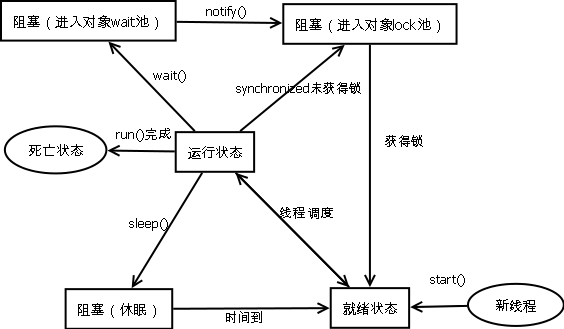
\includegraphics[width=\textwidth]{image/thread.png}
	\caption{线程状态生命周期图}
\end{figure}
\begin{enumerate}
	\item 诞生状态:线程刚被创建
	\item 就绪状态:线程的start方法已被执行,线程已准备好运行
	\item 运行状态:处理机分配给线程,线程正在运行
	\item 阻塞状态:
	\subitem 在线程发出输入输出请求且必须等待其返回
	\subitem 遇到synchronized标记的方法而未获得锁
	\subitem 为等候一个条件变量,线程调用wait()方法
	\item 休眠状态:执行sleep方法进入休眠
	\item 死亡状态:线程完成或退出
\end{enumerate}
\subsection{死锁}
线程在运行过程中,其中某个步骤往往需要满足一些条件才能继续进行下去,如果这个条件不能满足,
线程将在此步骤出现阻塞。
\par 如线程A等B,B等C,C又等...最后回到A,任何线程不能执行,造成死锁(deadlock)。
\subsection{控制线程的生命}
结束线程的生命:
\begin{itemize}
	\item 可控制run方法中循环条件方式来结束一个线程
	\item 使用stop结束线程生命
	\subitem 但如果一个线程正在操作共享数据段,操作过程没有完成就用stop结束的话,
	将会导致数据不完整。
\end{itemize}
\section{线程的调度}
\subsection{线程的优先级}
线程调度
\begin{enumerate}
	\item 在但CPU的系统中,多个线程需要共享CPU,在任何时间点上实际只能有一个线程在运行;
	\item 控制多个线程在同一个CPU上以某种顺序运行称为线程调度;
	\item Java虚拟机支持一种非常简单的、确定的调度算法——固定优先级算法,基于线程优先级对其进行调度;
	\item 每个Java线程都有一个优先级,范围1-10,默认为5;
	\item 在线程A中创建B,则B初始优先级和A相同;
	\item 如果A为后台线程,B也为后台线程;
	\item 可在线程创建后任何时刻,通过setPriority(int priority)改变优先级;
\end{enumerate}
\par 基于优先级线程调度
\begin{enumerate}
	\item 高优先级线程比低优先级先执行;
	\item 对相同优先级,Java处理是随机的;
	\item 底层操作系统支持优先级可能小于10,这会造成一些混乱,只能使用优先级作为
	作为粗略工具,最后可以通过yield()完成。
\end{enumerate}
\par 线程优先级队列
\par 如果某线程正在运行,则只有出现以下情况之一,才会暂停执行
\begin{itemize}
	\item 一个更高优先级线程处于就绪状态;
	\item 由于输入输出、调用sleep、wait、yield使其阻塞;
	\item 对于支持时间分片,时间分片执行完。
\end{itemize}
\par 注:
\begin{enumerate}
	\item JVM本身不支持某个线程抢夺另一个正在执行的线程具有同优先级的执行权;
	\item yield()会使正运行线程放弃执行,同优先级线程有机会调度,低优先级仍会被忽略。
\end{enumerate}